\documentclass[british, svgnames, dvipsnames]{upb-beamer}
\usepackage[export]{adjustbox}
\usepackage[justification=centering, font=normalsize, labelfont={normalsize,bf}]{caption}
\usepackage{mathtools, amssymb, bm}
\usepackage{booktabs}
\usepackage{multirow}
\usepackage{subcaption}
\usepackage[style=american]{csquotes}
\usepackage[newfloat]{minted}
\usepackage{fontspec}

\usemintedstyle{perldoc}
\defaultfontfeatures[JetBrainsMono]{
    Path=./fonts/mono/,
    Extension = .ttf,
    UprightFont=*-Medium,
    BoldFont=*-Bold,
    ItalicFont=*-Italic,
    BoldItalicFont=*-BoldItalic
}
\newfontfamily{\jbmono}[NFSSFamily=JetBrainsMono]{JetBrainsMono}
\newenvironment{codesnip}{\captionsetup{type=listing}\vspace{\intextsep}}{\vspace{\intextsep}} % Code magic
\SetupFloatingEnvironment{listing}{name=Code Snippet}
\definecolor{codebg}{rgb}{0.95,0.95,0.95}

\setbeamertemplate{caption}[numbered]


% --------------------------------------------------- %
%                  Presentation info	              %
% --------------------------------------------------- %

\title[The Shortcut Problem]{\textbf{\huge{The Shortcut Problem}}}
\author[Cristian Cristea]{\large{Performance Analysis and Optimisation Project\\[0.5cm]\textbf{Cristian Cristea}}}
\institute[UNSTPB -- ETTI]{\small{Faculty of Electronics, Telecommunications and Information Technology\\[0.5mm]National University of Science and Technology POLITEHNICA Bucharest}}
\date{June 2024}

\setbeamersize{text margin left=5mm,text margin right=5mm} 

\graphicspath{{img/}}

% --------------------------------------------------- %
%                    Title + Schedule                 %
% --------------------------------------------------- %

\begin{document}

\begin{frame}
    \titlepage
    \makebox[0.91\paperwidth]{
        \centering
        
\includegraphics[width=1.4cm,keepaspectratio]{upb.eps}
        \hfill
        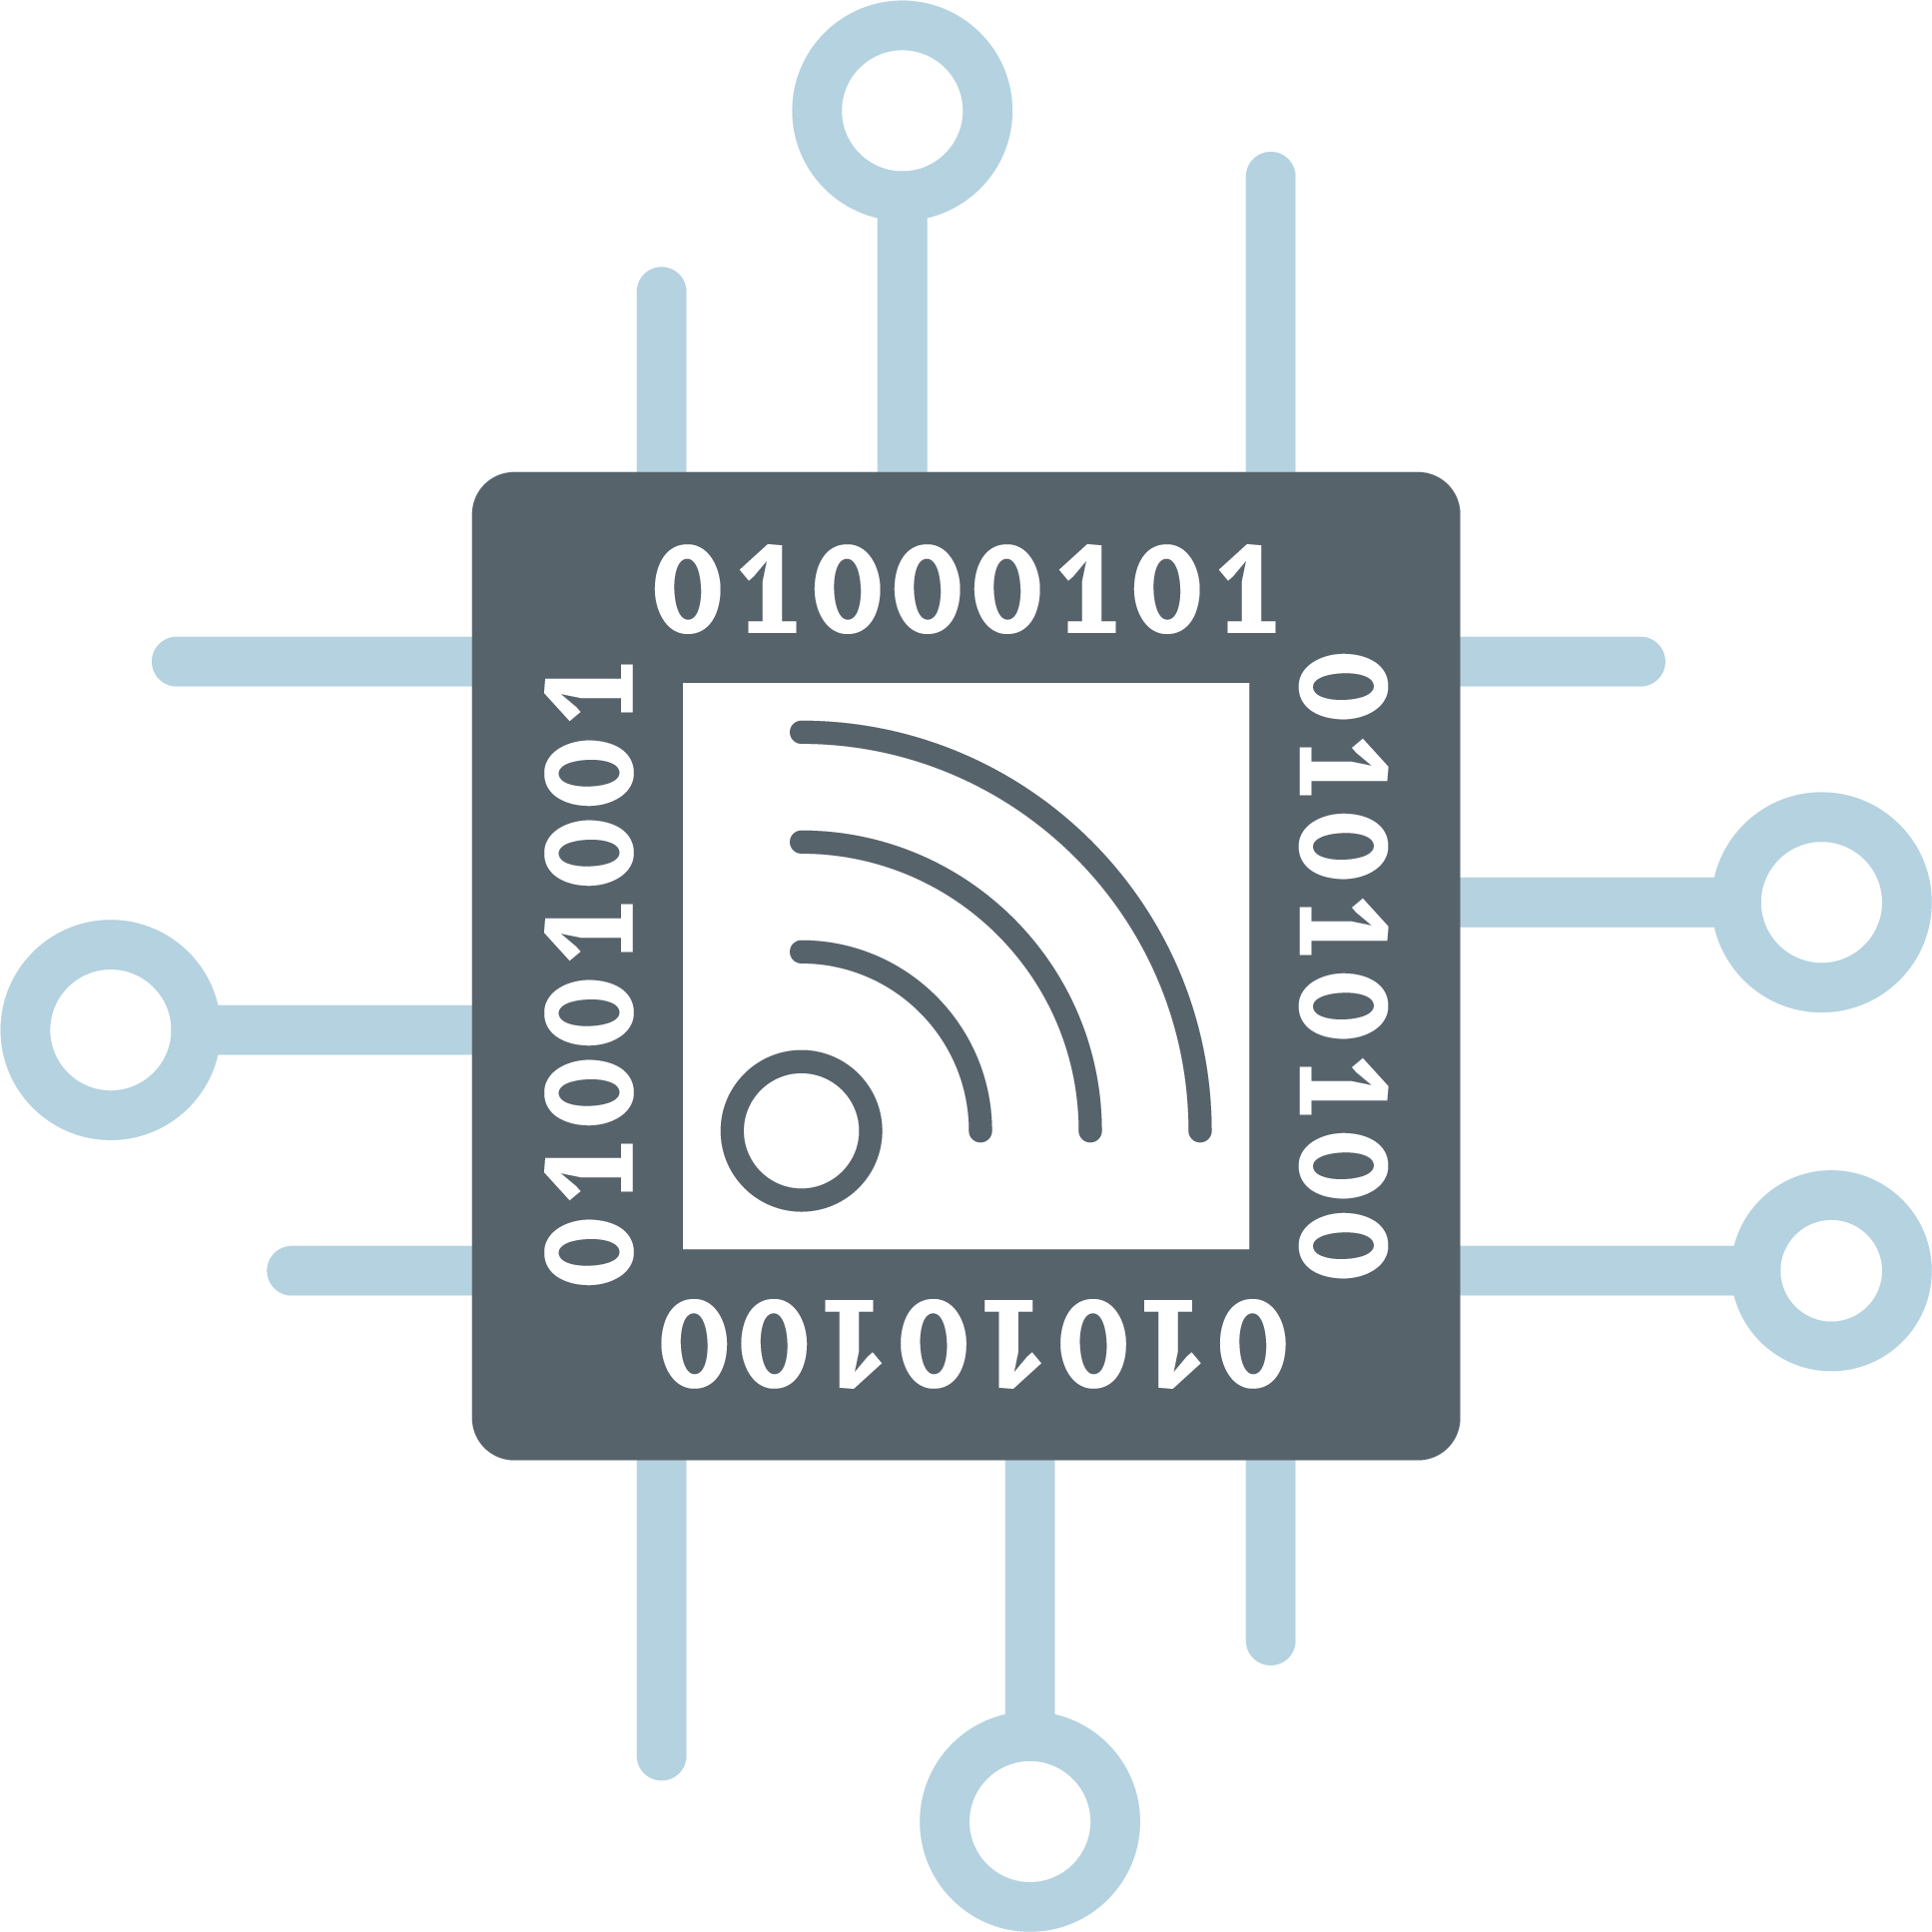
\includegraphics[width=1.4cm,keepaspectratio]{etti.png}%
    }%
\end{frame}

\begin{frame}{Table of Contents}
    \large{\tableofcontents}
\end{frame}

% --------------------------------------------------- %
%                    Presentation                     %
% --------------------------------------------------- %

% =================================================== %
\section{General Information}
% =================================================== %

\begin{frame}{Problem Description}
    We have a directed graph with $n$ nodes. The graph nodes are labelled with numbers $0, 1, \dots, n - 1$. There is a directed edge between each pair of nodes. The cost of the edge between nodes $i$ and $j$ is $d_{ij}$. We will assume that $d_{ij}$ is a non-negative real number. For convenience, we write $d_{ii}=0$ for each node $i$.
    \\~\\
    However, the costs do not necessarily satisfy the triangle inequality. We might have an edge of cost $d_{ij}=10$ from node $i$ to $j$, but there might be an intermediate node $k$ with $d_{ik}=2$ and $d_{kj}=3$. Then we can follow the route $i \rightarrow k \rightarrow j$ at a total cost of $2 + 3 = 5$, while the direct route $i \rightarrow j$ would cost $10$.
    \\~\\
    The task is to find for all $i$ and $j$ what is the cost of getting from $i$ to $j$ by taking \textbf{at most two edges}. If we write $r_{ij}$ for the result, then
    
    $$r_{ij} = \min_k (d_{ik} + d_{kj})\,,$$
    
    where $k$ ranges over $0, 1, \dots, n - 1$. Note that routes such as $i \rightarrow i \rightarrow j$ will also be considered, hence a path of one edge will be found if it happens to be the cheapest.
\end{frame}

\begin{frame}{Problem Description}
    \begin{figure}[h!]
        \centering
        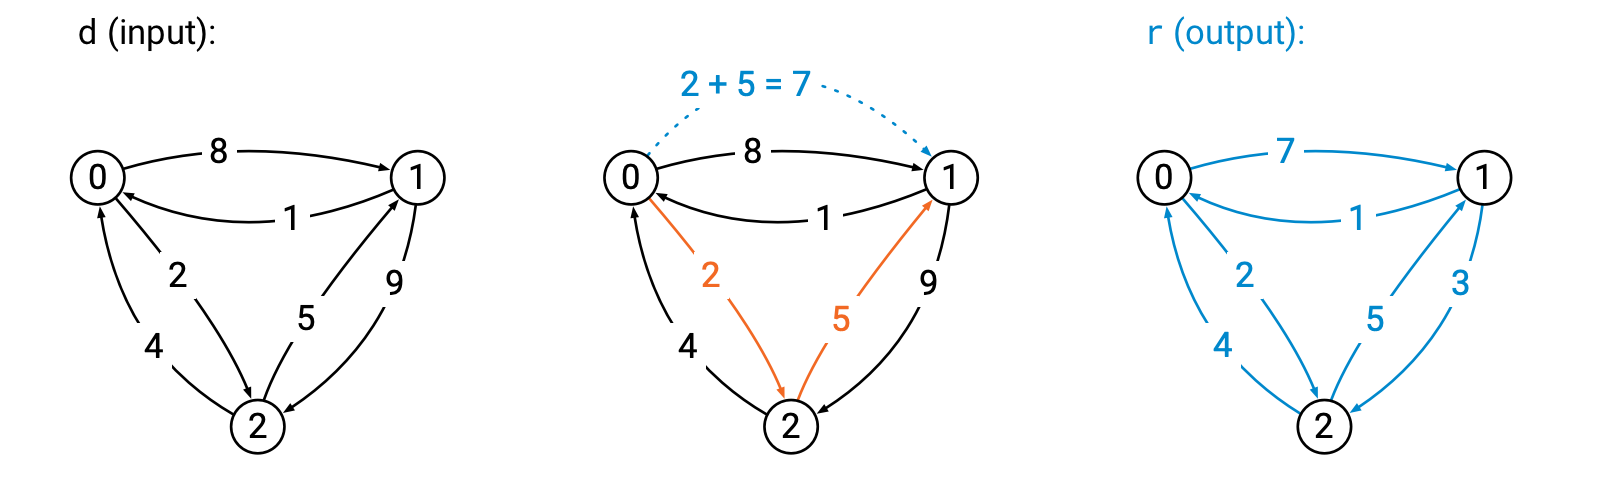
\includegraphics[width=\linewidth]{img/graphs.png}
        \caption{Graph Example}
        \label{fig:graphs}
    \end{figure}
\end{frame}

% =================================================== %
\section{Progress}
% =================================================== %

\begin{frame}[fragile]{Straightforward (naive) implementation}
\begin{codesnip}
\begin{minted}[fontsize = \small, baselinestretch = 0.9, framesep = 5pt, bgcolor = codebg, breaklines = true, codetagify = true, fontfamily = JetBrainsMono]{cpp}
template <typename T>
auto Shortcut(Graph<T> const & graph) -> Graph<T>
{
    Graph<T> result{graph.size()};

    for (std::size_t row = 0; row < graph.size(); ++row)
    {
        for (std::size_t col = 0; col < graph.size(); ++col)
        {
            T minimum{max_value<T>::get()};
            
            for (std::size_t k = 0; k < graph.size(); ++k)
            {
                minimum = std::min(minimum, graph[row, k] + graph[k, col]);
            }

            result[row, col] = minimum;
        }
    }

    return result;
}
\end{minted} 
\caption{Naive C++ implementation}
\end{codesnip}
\end{frame}

\begin{frame}{Implementations}
    \begin{itemize}
        % \setlength\itemsep{0.5cm}
        \pause
        \item \textbf{Naive} -- The straightforward approach which establishes the baseline for benchmarking the other implementations.
        \pause
        \item \textbf{NaiveOpenMP} -- The improved baseline approach which just distributes the work across all threads using \texttt{OpenMP}.
        \pause
        \item \textbf{Cached} -- The matrix of the graph is accessed in a cache-friendly manner by rows but inefficiently by columns. To address this issue, the matrix is transposed, ensuring that both row and column accesses are optimised for cache efficiency.
        \pause
        \item \textbf{CachedOpenMP} -- The Cached implementation which just distributes the work across all threads using \texttt{OpenMP}.
        \pause
        \item \textbf{SIMD} -- To leverage the CPU's SIMD instructions, the matrix elements of the graph are stored as vector types and padded as necessary. Additionally, the transposed approach is employed to optimise cache access.
        \pause
        \item \textbf{SIMDOpenMP} -- The SIMD implementation which just distributes the work across all threads using \texttt{OpenMP}.
        \pause
        \item \textbf{OpenCL} -- The straightforward approach was implemented as an \texttt{OpenCL} kernel.
        \pause
        \item \textbf{OpenCLSwapped} -- The same straightforward \texttt{OpenCL} kernel was used, but with the row and column indices swapped to enhance cache access efficiency.
    \end{itemize}
\end{frame}

% =================================================== %
\section{Results}
% =================================================== %

\begin{frame}{Results}
    \begin{table}[h]
    \resizebox{\textwidth}{!}{%
    \begin{tabular}{lrrrrrr}
    \toprule
     \textbf{Implementation} & $\bm{N = 100}$ & $\bm{N = 200}$ & $\bm{N = 500}$ & $\bm{N = 1000}$ & $\bm{N = 2000}$ & $\bm{N = 5000}$\\
     \midrule
     Naive & 0 ms & 5 ms & 70 ms & 1 065 ms & 40 961 ms & 974 426 ms \\
     NaiveOpenMP & 20 ms & 20 ms & 45 ms & 315 ms & 8 667 ms & 172 436 ms \\
     Cached & 0 ms & 2 ms & 33 ms & 265 ms & 2 888 ms & 41 513 ms \\
     CachedOpenMP & 30 ms & 30 ms & 30 ms & 71 ms & 672 ms & 13 703 ms \\
     SIMD & 0 ms & 5 ms & 50 ms & 317 ms & 3 213 ms & 42 535 ms \\
     SIMDOpenMP & 30 ms & 30 ms & 40 ms & 127 ms & 596 ms & 9 735 ms \\
     OpenCL & 0 ms & 0 ms & 6 ms & 59 ms & 1 823 ms & 40 173 ms \\
     OpenCLSwapped & 0 ms & 0 ms & 1 ms & 31 ms & 290 ms & 4 672 ms \\
     \cmidrule{1-7}
     SoA & 0 ms & 0 ms & 0 ms & 7 ms & 271 ms & 6 453 ms \\
     SoAOpenMP & 20 ms & 20 ms & 20 ms & 22 ms & 77 ms & 1 162 ms \\
     SoAOpenCL & 0 ms & 0 ms & 0 ms & 1 ms & 8 ms & 122 ms \\
     \bottomrule
    \end{tabular}
    }
    \caption{Results comparison for different input sizes}
    \label{tab:ref}
    \end{table}
\end{frame}

\begin{frame}{Conclusions}
    \begin{itemize}
        \setlength\itemsep{0.5cm}
        \pause
        \item \textbf{Distributing Computation Load} -- Utilising APIs like \texttt{OpenMP} to distribute the computation load across multiple threads significantly increases speed. However, this approach introduces some latency due to thread spawning and context switching times.
        \pause
        \item \textbf{Optimising Memory Access} -- Maintaining a high rate of cache hits is crucial for performance optimisation since memory access is often the primary bottleneck in computational processes.
        \pause
        \item \textbf{Leveraging CPU SIMD Instructions} -- Exploiting all CPU resources, including SIMD instruction extensions, enhances performance by taking advantage of parallel processing capabilities inherent in these instructions.
        \pause
        \item \textbf{Utilising Specialised Hardware} -- Delegating the processing of parallel programs to specialised hardware such as GPUs significantly reduces computation time due to the massive parallelism these devices offer.
        \pause
        \item \textbf{Advanced Performance Techniques} -- Achieving state-of-the-art performance requires employing advanced techniques. For CPUs, this includes strategies like register reuse and prefetching. For GPUs, optimising data reuse in shared memory is essential for maximising performance.
    \end{itemize}
\end{frame}

\begin{frame}
    \hfill\Huge{Thank you for your attention! Questions?}
    \color{structure.fg!75!black}{\rule{\textwidth}{0.05cm}}
\end{frame}

\end{document}
